% !TeX spellcheck = da_DK
\subsection{Referencespænding til Komparator}\label{subsec:Spaendingsref_Komparator}
\subsubsection{Teori og design}
Der skal til komparatorblokken forsynes med en konstant spænding, da denne skal anvendes som sammenligningsgrundlag ift. inputsignalet. Her anvendes igen en referencespænding, som er beskrevet i afsnit \ref{subsec:Spaendingsref} på side \pageref{subsec:Spaendingsref}. Der anvendes samme referencediode til denne referencespænding, som kan ses på \figref{fig:Spaendingsreference} på side \pageref{subsec:Spaendingsref}. \\
For at udregne modstanden R1 for referencespændingen til komparatoren benyttes \eqref{eq:udregning_modstand}. Den ønskede referenceværdi er $2.5$V, så der skal i dette tilfælde ikke benyttes en spændingsdeler. I starten af kredsløbet indsættes en operations forstærker (TL$082$), som har to input og output. \cite{Corporation2013} Derved kan denne fungere som buffer, beskrevet i bilag \ref{Bilag:Pilotforsoeg} på side \pageref{Bilag:Pilotforsoeg}, til komparator kredsløbet og en inverterende forstærker.\cite{Schaumann2014} Da spændingen går direkte ind i bufferen, er den maksimale biasstrøm på $50nA$. Biasstrømmen for referencedioden er igen sat til $200\mu$A. Dermed kan værdierne indsættes i formlen og R1 kan beregnes:
\begin{equation}
R_komparator = \frac{5.5V-2.5V}{50nA + 200\mu\text{A}} = 14999.62501\Omega \approx 15K\Omega 
\end{equation} 
Operationsforstærkeren TL$082$ benyttes som nævnt som en buffer og inverterende forstærker, da der både ønskes et positivt og negativt output til tærskelværdierne i komparatorblokken.
\begin{figure}[H]
	\centering
	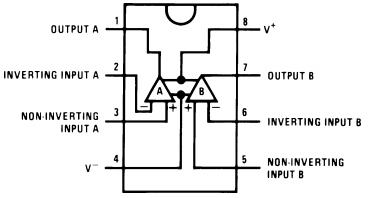
\includegraphics[scale=0.65]{figures/cProblemloesning/TL082.PNG}
	\caption{På figuren ses pinkonfigurationen af operationsforstærkeren TL$082$. Det positive output til komparatorblokken vil komme fra pin $1$ altså output A, og det negative output til komparatorblokken vil komme fra pin $7$ altså output B. \cite{Corporation2013}}
	\label{fig:TL082}
\end{figure}
\noindent Der vides fra teorien, at der skal benyttes to modstande til designet af en inverterende forstærker. Da der ønskes et gain på 1, skal disse to modstande have samme værdi. \cite{Nilsson2011} Designet af referencespændingen med operationsforstærkeren TL$082$ ses på \figref{fig:ref_komparator}.

\begin{figure}[H]
	\centering
	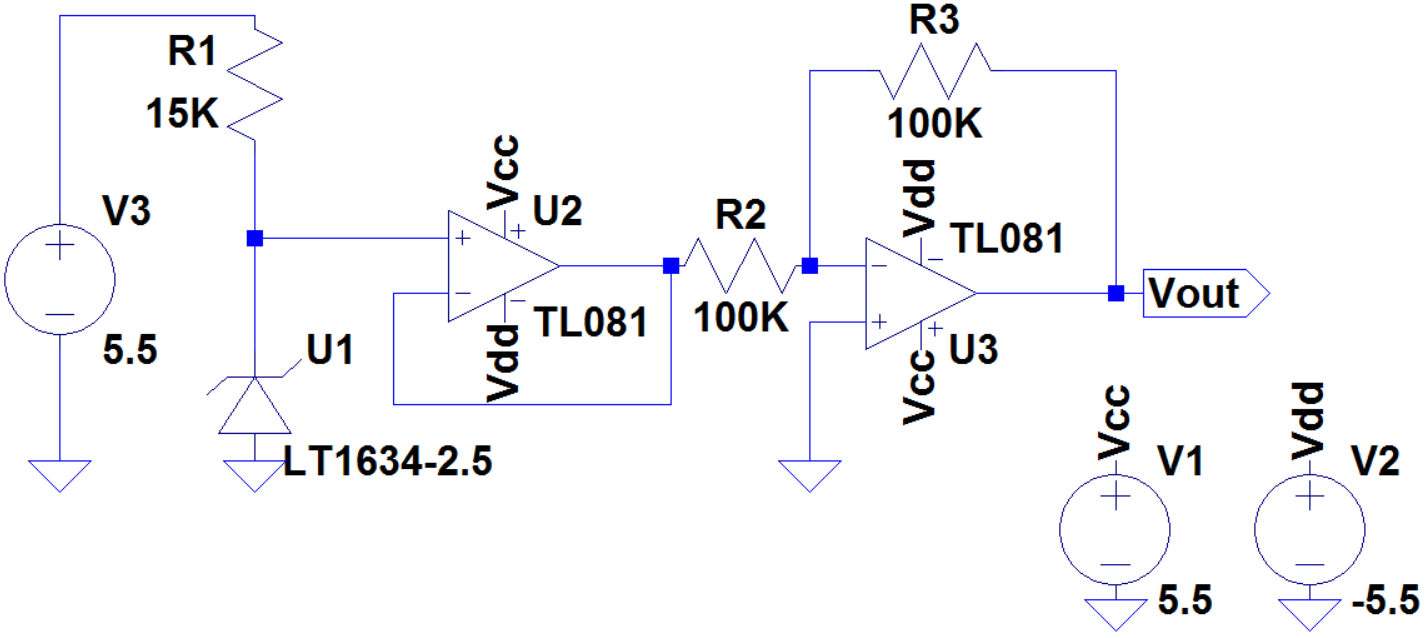
\includegraphics[scale=0.4]{figures/cProblemloesning/Reference_komparator.PNG}
	\caption{På figuren ses designet af referencespændingsblokken, der skal levere en referencespænding til komparatorblokken. Operationsforstærkeren TL$082$ fungerer som to TL$081$'ere, og derfor er simuleringen opbygget således. \cite{Corporation2013}}
	\label{fig:ref_komparator}
\end{figure}

\subsubsection{Simulering}
Der foretages en simulering i LTspice, for at se, om designet fungerer ideelt og hvor præcis spændingsreferencen er. Resultatet af simuleringen ses i \tableref{Tab:SpaendigsRef_komparator}

\begin{table}[H]
\centering
\begin{tabular}{|l|l|l|l|}\hline
	& \textit{\begin{tabular}[c]{@{}l@{}}Forventet\\outputsignal\end{tabular}} & \textit{\begin{tabular}[c]{@{}l@{}}Målte\\outputsignal\end{tabular}} & \textit{Afvigelse} \\ \hline
	\textit{Input fra spændingsforsyning}      & $5.5$V             &  $5.5$V       &   $0\%$         \\ \hline
	\textit{Output fra spændingsreference}     & $2.5$V             &  $2.5007$V    &   $0.03 \%$    \\ \hline
	\textit{Output A fra TL082} &  $2.5$V            &   $2.5006$V   &   $0.02\%$    \\ \hline
	\textit{Output B fra TL082} & -$2.5$V            &  -$2.5006$V   &   $0.02\%$    \\ \hline
\end{tabular}
\caption{I tabellen ses resultaterne fra simuleringen i LTspice af spændingsreferencen med operationsforstærkeren til komparatoren.}
\label{Tab:SpaendigsRef_komparator}
\end{table}
\noindent I \tableref{Tab:SpaendigsRef_komparator} ses det, at der er en lav afvigelse mellem det forventede output og det simulerede output. Dette forventes, da der benyttes ideelle komponenter i LTspice. Derved fungerer kredsløbet teoretisk og kan implementeres. På \figref{fig:Spaendingsreference_komparator_sim} ses simuleringen af spændingsreferencen og operationsforstærkeren.
\begin{figure}[H]
	\centering
	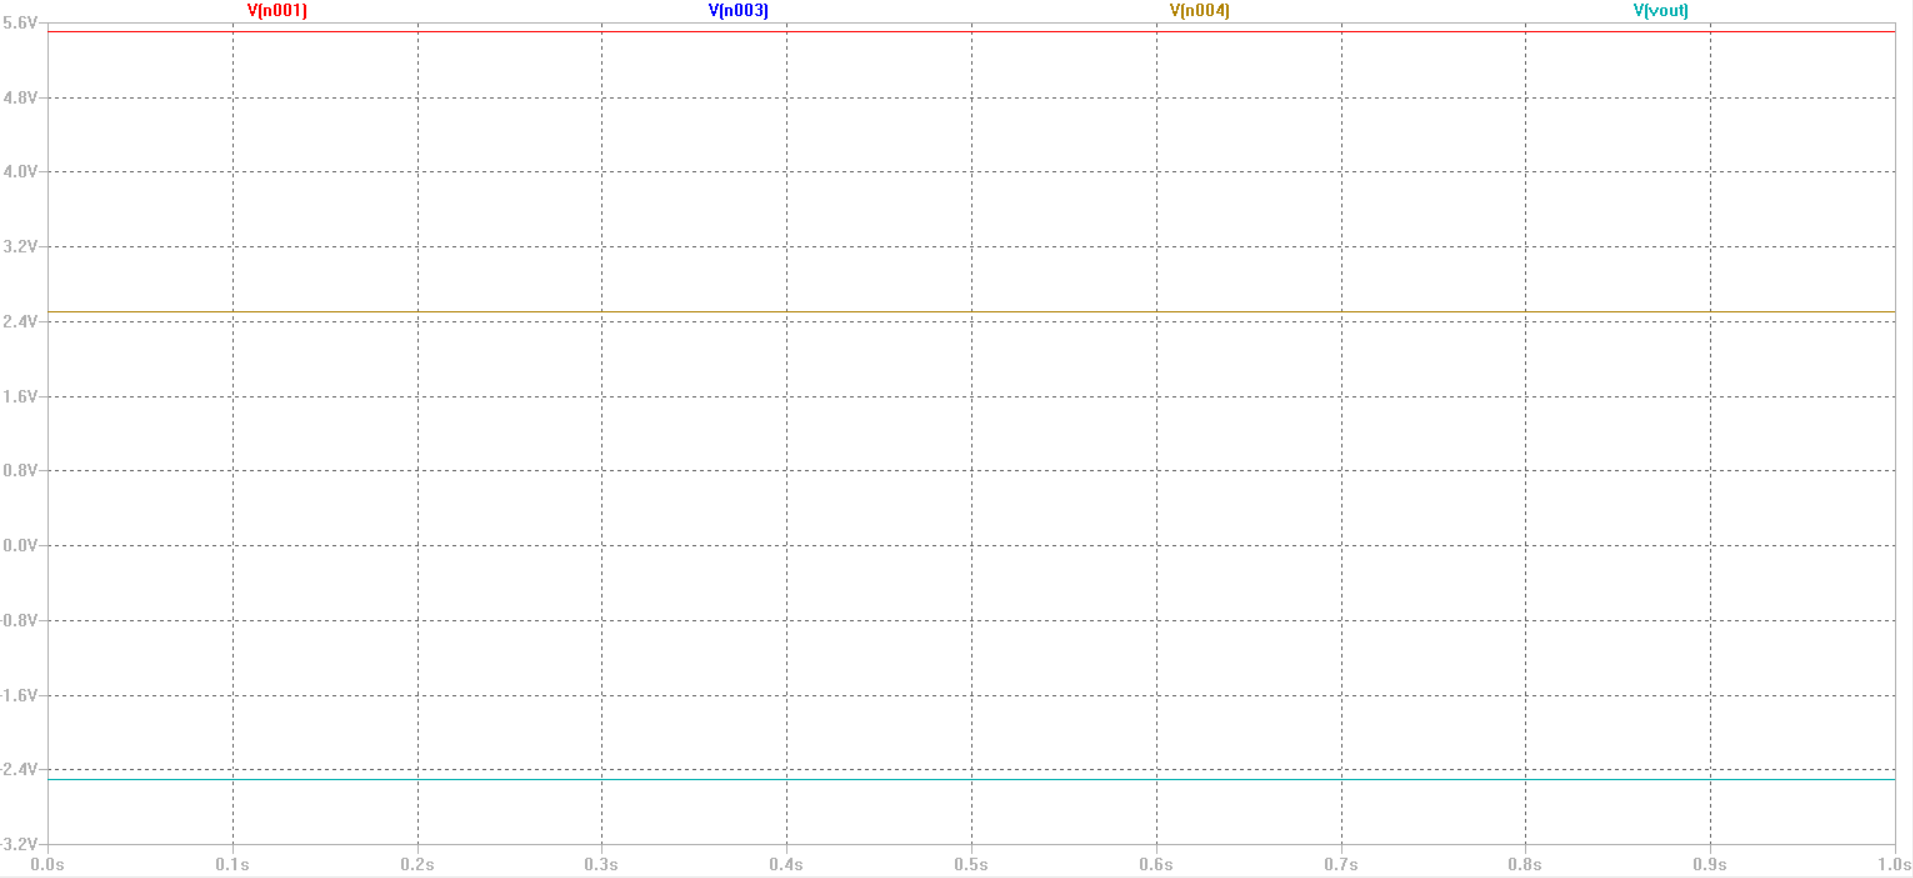
\includegraphics[scale=.3]{figures/cProblemloesning/Reference_sim_kompar.PNG}
	\caption{På figuren ses, at inputtet er $5.5$V, outputtet fra spændingsreferencen er $2.5$V, hvilket output A for TL$082$ også er. Derfor kan man kun se output A på figuren, da de ligger oveni hinanden. Output B fra spændingsdeleren er -$2.5$V.}
	\label{fig:Spaendingsreference_komparator_sim}
\end{figure}
\subsubsection{Implementering og test}
I implementeringen arbejdes der med reelle komponenter. Derfor antages det, at der kan være afvigelser fra resultaterne imellem testen med ideelle komponenter i dette afsnit og testen med reelle komponenter i simuleringen. \\
Der ses på \figref{fig:ref_komparator}, at der skal benyttes tre modstande på hhv. $15$K$\Omega$, $100$K$\Omega$ og $100$K$\Omega$ til opbygningen af spændingsreferencen og spændingsdeleren til offsettet. Disse blev målt inden testen, hvilket fremgår i \tableref{Tab:modstand_Kompar}.

\begin{table}[H]
	\centering
	\begin{tabular}{|l|l|l|}
		\hline
		\textit{Teoretisk} & \textit{Ved måling} & \textit{\% afvigelse} \\ \hline
		$15$K$\Omega$       & $14.9983$K$\Omega$   & $0.01$\%               \\ \hline
		$100$K$\Omega$      & $99.631$K$\Omega$    & $0.37$\%               \\ \hline
		$100$K$\Omega$      & $99.681$K$\Omega$    & $0.32$\%               \\ \hline
	\end{tabular}
	\caption{I tabellen ses der, at alle tre modstande afviger lidt fra deres teoretiske værdi, hvilket er forventet af reelle komponenter. Kravet til disse fire modstande var dog, at de maks må afvige fra deres teoretiske værdi med $\pm1\%$ jævnfør afsnit \ref{Ref_Offset_Afs} på side \pageref{Ref_Offset_Afs}. Disse modstande accepteres derfor.}
	\label{Tab:modstand_Kompar}
\end{table}
\noindent Herefter implementeres kredsløbet. Til aflæsning af spændingsniveauerne anvendes et multimeter. De aflæste resultater står i \tableref{Tab:SpaendingsRef_kompar_test}.
\begin{table}[H]
	\centering
	\begin{tabular}{|l|l|l|l|} \hline
		& \textit{\begin{tabular}[c]{@{}l@{}}Forventet\\outputsignal\end{tabular}} & \textit{\begin{tabular}[c]{@{}l@{}}Målte\\outputsignal\end{tabular}} & \textit{Afvigelse} \\ \hline
		\textit{Input fra spændingsforsyning}       & $5.5$V    & $5.5530$V  & $0.96\%$ \\ \hline
		\textit{Output fra spændingsreference}      & $2.5$V    & $2.5166$V  & $0.66\%$ \\ \hline
		\textit{Output A fra TL081}                 & $2.5$V    & $2.5157$V  & $0.63\%$ \\ \hline
		\textit{Output B fra TL081}                 & -$2.5$V   & -$2.5245$V & $0.98\%$ \\ \hline
	\end{tabular}
	\caption{I tabellen ses en oversigt over de forventede og målte outputsignaler fra testen for spændingsreferencen og operationsforstærkeren TL$082$ til komparatorblokken.}
	\label{Tab:SpaendingsRef_kompar_test}
\end{table}
\noindent Der ses ud fra resultaterne i \tableref{Tab:SpaendingsRef_offset_test}, at blokken overholder kravene fra afsnit \ref{Ref_Kompar_Afs} på side \pageref{Ref_Kompar_Afs}. Derudover ligger afvigelserne indenfor tolerancerne. \\
Der tages ikke hensyn til outputimpedansen fra denne blok, da operationsforstærkeren, som fungerer som en buffer, sørger for, at outputimpedansen bliver tilstrækkelig lav til ikke at have en betydning.